\documentclass{article}
\usepackage[utf8]{inputenc}
\usepackage[T1]{fontenc}
\usepackage[french]{babel}
\usepackage{graphicx}
\usepackage{geometry}
\usepackage{multirow}

\title{Les mesures sociosanitaires ont-elles affecté la collaboration entre étudiants ?}
\author{Jessica Coulombe \and Frédéric Laberge \and Laurie L'Espérance \and Arigna Luangphachaleun \and Olivier Whitter}
\date{25 Avril 2021}

\geometry{
letterpaper,
portrait,
left=30mm,
right=30mm,
top=30mm,
bottom=40mm
}

\begin{document}

\maketitle

\begin{abstract}
    La covid-19 a bouleversé le monde entier. Plusieurs milliers de personnes se sont retrouvées confinées à la maison. L’Université de Sherbrooke n’a pas été épargnée par le virus. La majorité des cours présentiels ont été remplacés par des cours à distance. Ce travail avait comme objectif de vérifier si les mesures sociosanitaires contre la covid-19 ont affecté les collaborations entre étudiants universitaires. Le nombre de collaborations par étudiant semble inférieur après le début de la pandémie qu’avant. Toutefois, certains cours favorisent davantage la collaboration que d’autres, ce qui pourrait influencer les résultats. Il n’a pas été possible de confirmer une relation de causalité entre le nombre de collaborations et le contexte pandémique.
\end{abstract}
\section*{Introduction}
    Autant chez les végétaux que chez les animaux, plusieurs espèces se retrouvent au sein d’une seule et même communauté. En écologie, les différentes interactions entre les espèces d’une communauté sont représentées dans un réseau écologique, où une interaction entre deux espèces constitue un lien \cite{landi_complexity_2018}. L’ensemble des liens est ensuite regroupé pour y former un réseau qui permet de décrire et de comparer les structures d’une communauté, mais aussi d’un écosystème \cite{bruder_importance_2019}. Les réseaux écologiques sont souvent utilisés lors de projets d’aménagement, notamment pour l’évaluation de la stabilité d’un écosystème en réponse à différents scénarios\cite{bruder_importance_2019}. Ce concept, quoique bien intégré en écologie, peut-il s’appliquer à un contexte social? Plus particulièrement, si les composantes d’une étude portent sur le nombre de collaborations entre les étudiants du baccalauréat en écologie, auront-elles les mêmes propriétés que celles d’un réseau écologique? Mais aussi, dans un contexte de pandémie où des mesures sociosanitaires ont été mises en place à l’Université de Sherbrooke afin de limiter la propagation de la covid-19, un changement majeur a été apporté au mode d’enseignement. Les cours traditionnellement offerts en mode présentiel ont dû être offerts à distance, ce qui pourrait avoir un impact sur le réseau de collaboration entre les étudiants. L’objectif de ce travail est de faire un portrait du réseau de collaborations entre les étudiants et d’évaluer les effets de la méthode d’enseignement sur celui-ci.

\section*{Méthodologie}

\subsection*{Base de données}
    Les données ont été collectées auprès des étudiants du baccalauréat en écologie participant au cours de biologie computationnelle (BIO500) à la session d’hiver 2021 (H21). L’échantillonnage a été réalisé durant mars 2021 en demandant aux étudiants de compléter une base de données prédéfinie avec le logiciel Microsoft Excel. La base de données brutes est composée de trois tables, soit la table \textsc{nœuds}, la table \textsc{collaborations} et la table \textsc{cours}.\\
    La table \textsc{nœuds} comporte toutes les informations concernant les étudiants qui font partie des réseaux de collaborations des étudiants du cours BIO500, dont le nom complet de l’étudiant et s’il est inscrit au cours BIO500 à la session d’hiver 2021. La clé primaire de cette table est le nom complet de l’étudiant.\\
    La table \textsc{collaborations} décrit toutes les collaborations présentes et passées dans le parcours universitaire des étudiants échantillonnés. La clé primaire est composée de toutes les variables de la table, soit le nom et le prénom d’un premier étudiant, le nom et le prénom du second étudiant avec lequel le premier étudiant collabore, la session et le sigle du cours où la collaboration a lieu. À noter que les liens de collaboration sont unidirectionnels. Ainsi, il y a deux liens pour chaque paire d’étudiants qui ont travaillé ensemble à un moment donné.\\
    La table \textsc{cours} contient plusieurs informations pour chaque cours, dont le sigle du cours qui est la clé primaire de cette table et si le cours a été enseigné en présentiel ou à distance.

\subsection*{Réalisation des figures}
\subsubsection*{Figure \ref{fig:re}: Réseau}
    Afin d’épurer la figure, seule une partie du réseau a été sélectionnée pour la représentation visuelle. La figure \ref{fig:re} présente ainsi uniquement les collaborations entre les étudiants du cours BIO500. Pour ce faire, une requête SQL a fourni le nombre de collaborations pour chaque couple d'étudiants où les deux étudiants suivent le cours BIO500. Par la suite, une matrice d’adjacence a été créée avec les données fournit par la requête SQL précédente. Les lignes et les colonnes de la matrice représentent les différents étudiants et les données dans les cellules de la matrice sont le nombre de collaborations par paire d’étudiants. Cette matrice fut directement utilisée avec la librairie « igraph » dans le logiciel R pour générer la figure du réseau. L’algorithme permettant le placement des nœuds est celui de Kamada-Kawai. Finalement, une couleur a été associée à chaque nœud selon leur nombre de liens en utilisant la palette de couleur « heat ».
\subsubsection*{Figure \ref{fig:d}: Diagramme à bandes}
    Pour former la figure \ref{fig:d}, le nombre de collaborations de chaque cours a été divisé au nombre d’étudiants participant au cours, ce qui a donné le nombre de collaborations moyen par étudiant pour chaque cours. Un diagramme à bande a permis de visualiser les résultats en ordre décroissant avec les cours qui favorisent le plus la collaboration en haut.
\subsubsection*{Figure \ref{fig:h}: Histogrammes}
    Pour faire la figure \ref{fig:h}, le nombre de liens par étudiant a été compté avec la fonction \textsc{count} dans une requête SQL qui sélectionnait d’abord les collaborations de 2019 et avant des étudiants du cours BIO500. Cette requête a permis de créer l’histogramme d’avant covid-19. La même méthode a été utilisée pour former l’histogramme d’après covid-19 excepté qu’il comprend seulement les collaborations qui ont eu lieu en 2020 et après. Pour bien visualiser les résultats et comparer le nombre de collaborations pré et postcovid-19, les histogrammes ont été juxtaposés, plutôt que jumelés en un seul histogramme.

\section*{Résultats et Discussion}
    Il ne semble pas avoir de sous-groupes distincts dans le réseau de collaboration des étudiants (figure \ref{fig:re}). En effet, tous les étudiants du réseau sont connectés entre eux par quelques nœuds de distance (figure \ref{fig:re}). Il est important de prendre en considération que les bases de données ne contenaient pas tous les étudiants du cours BIO500, mais uniquement la moitié du groupe, puisque la classe était divisée en deux groupes pour respecter la distanciation sociale. C’est pourquoi certains étudiants participant à ce cours n’ont qu’une collaboration.
\begin{figure}[h]
\centering
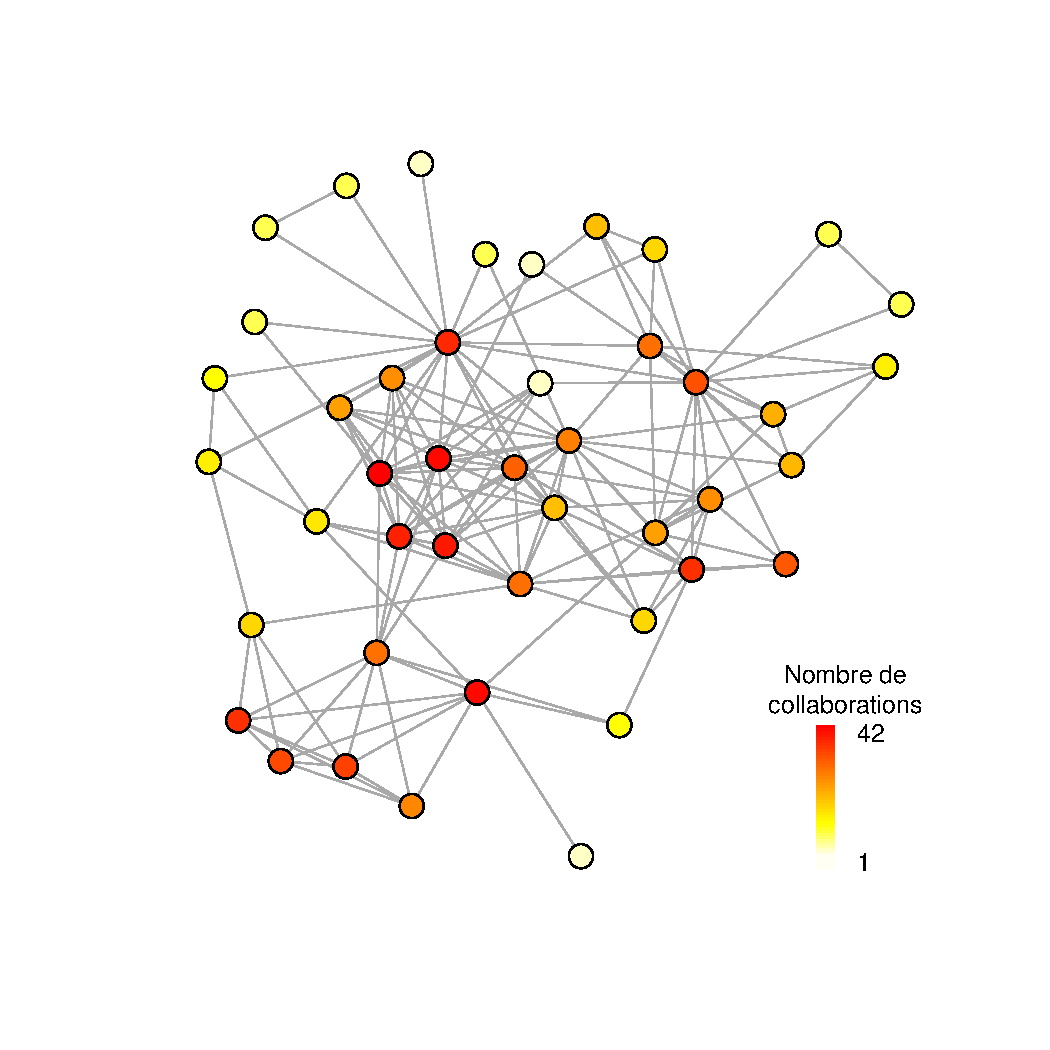
\includegraphics[width=0.5\textwidth]{figure_reseau_bio500.pdf}
\caption{Réseau de toutes les collaborations entre les étudiants inscrits au cours Méthode computationnelle (BIO500) à l'hiver 2021 qui ont lieu durant leur parcours universitaire.}
\label{fig:re}
\end{figure}
\hfill \break
    Le nombre de coéquipiers différents avec lesquels un étudiant collabore change peu entre les cours à distance et les cours en présentiel (tableau \ref{tab:coe}). Il semblerait qu’en général les étudiants n’ont pas collaboré avec moins de personnes différentes en télétravail. Toutefois, le nombre maximal de coéquipiers différents diminue de plus de la moitié en passant de cours en présentiel à des cours à distance (tableau). Ces résultats pourraient montrer que les cours à distance limitent le nombre de personnes différentes avec qui les étudiants travaillent, ce qui est préférable en temps de pandémie mondiale. Cependant, il n’est pas possible d’en conclure une relation de causalité. En effet, il est possible que cette tendance soit due à d’autres facteurs comme la progression du parcours universitaire des étudiants.
\hfill \break
\begin{table}[ht]
\caption{Nombre de coéquipiers différents que les étudiants ont eu en enseignement en présentiel et à distance. }
\label{tab:coe}
\centering
\begin{tabular}{|c|c|c|c|}
    \hline
    \multirow{2}{*}{Cours}&\multicolumn{3}{c|}{Nombre de coéquipiers}\\
    \cline{2-4}
    &Minimum&Moyenne&Maximum\\
    \hline
    Présentiel&1&6&24\\
    \hline
    Distance&1&4&11\\
    \hline
\end{tabular}
\end{table}

\hfill \break   
    Comme représenté dans la figure \ref{fig:d}, certains cours comme BCL606 favorisent grandement la collaboration entre étudiants avec la formation de grandes équipes de travail de 8 étudiants, alors que d’autres cours forment des équipes de 2 tels que ECL611 ou ECL603 (figure \ref{fig:d}).
\hfill \break
\begin{figure}[h]
\centering
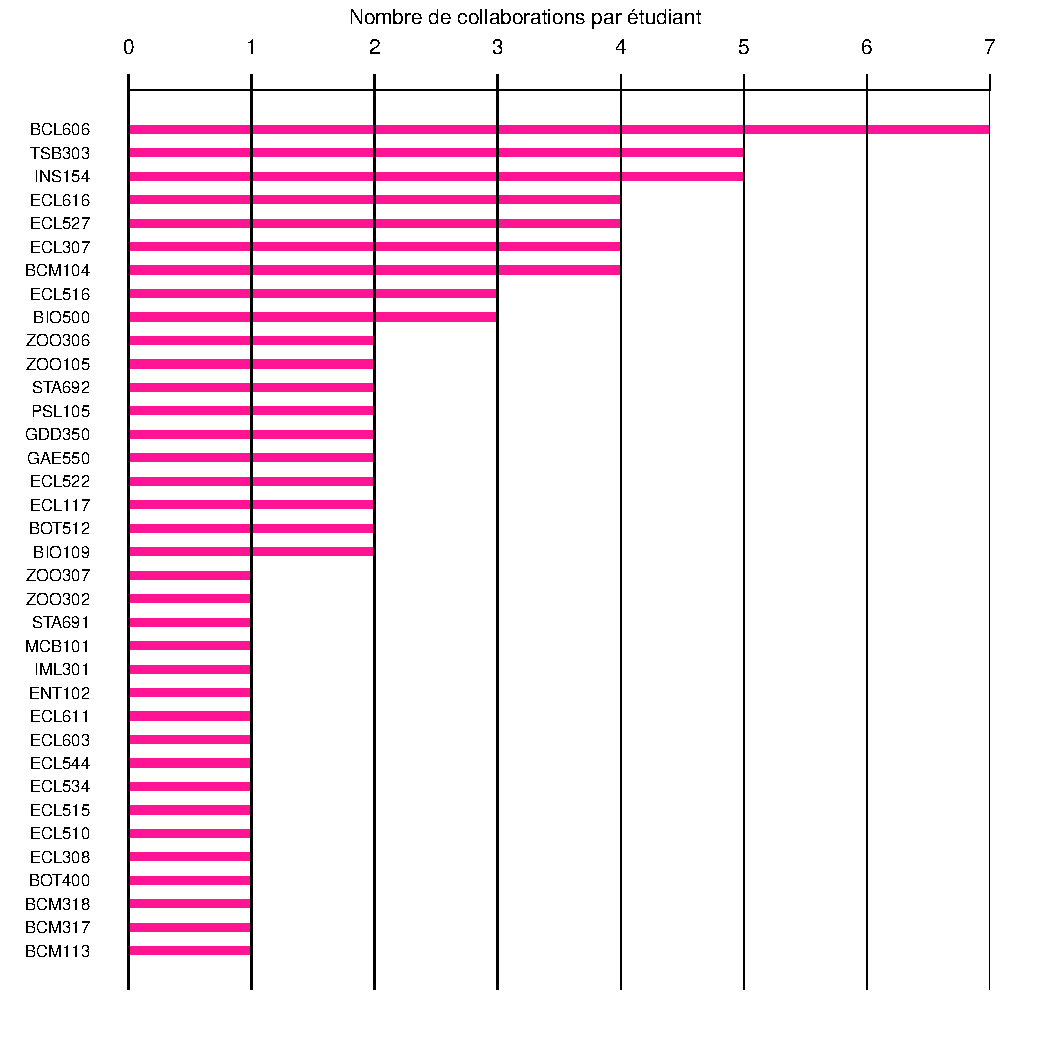
\includegraphics[width=0.90\textwidth]{figure_collaborations_etudiant.pdf}
\caption{Nombre de collaborations par étudiants pour chaque cours où il y a eu des collaborations}
\label{fig:d}
\end{figure}
\clearpage
    Avant la mise en place de mesures sociosanitaires en 2020 pour freiner la propagation de la covid-19, il semblerait que le nombre de collaborations par étudiant était distribué plus aléatoirement qu’après l’établissement de ces règles où la plupart des étudiants ont 10 collaborations et moins (figure \ref{fig:h}). Le contexte pandémique pourrait avoir affecté les collaborations entre les étudiants universitaires.
\begin{figure}[h]
\centering
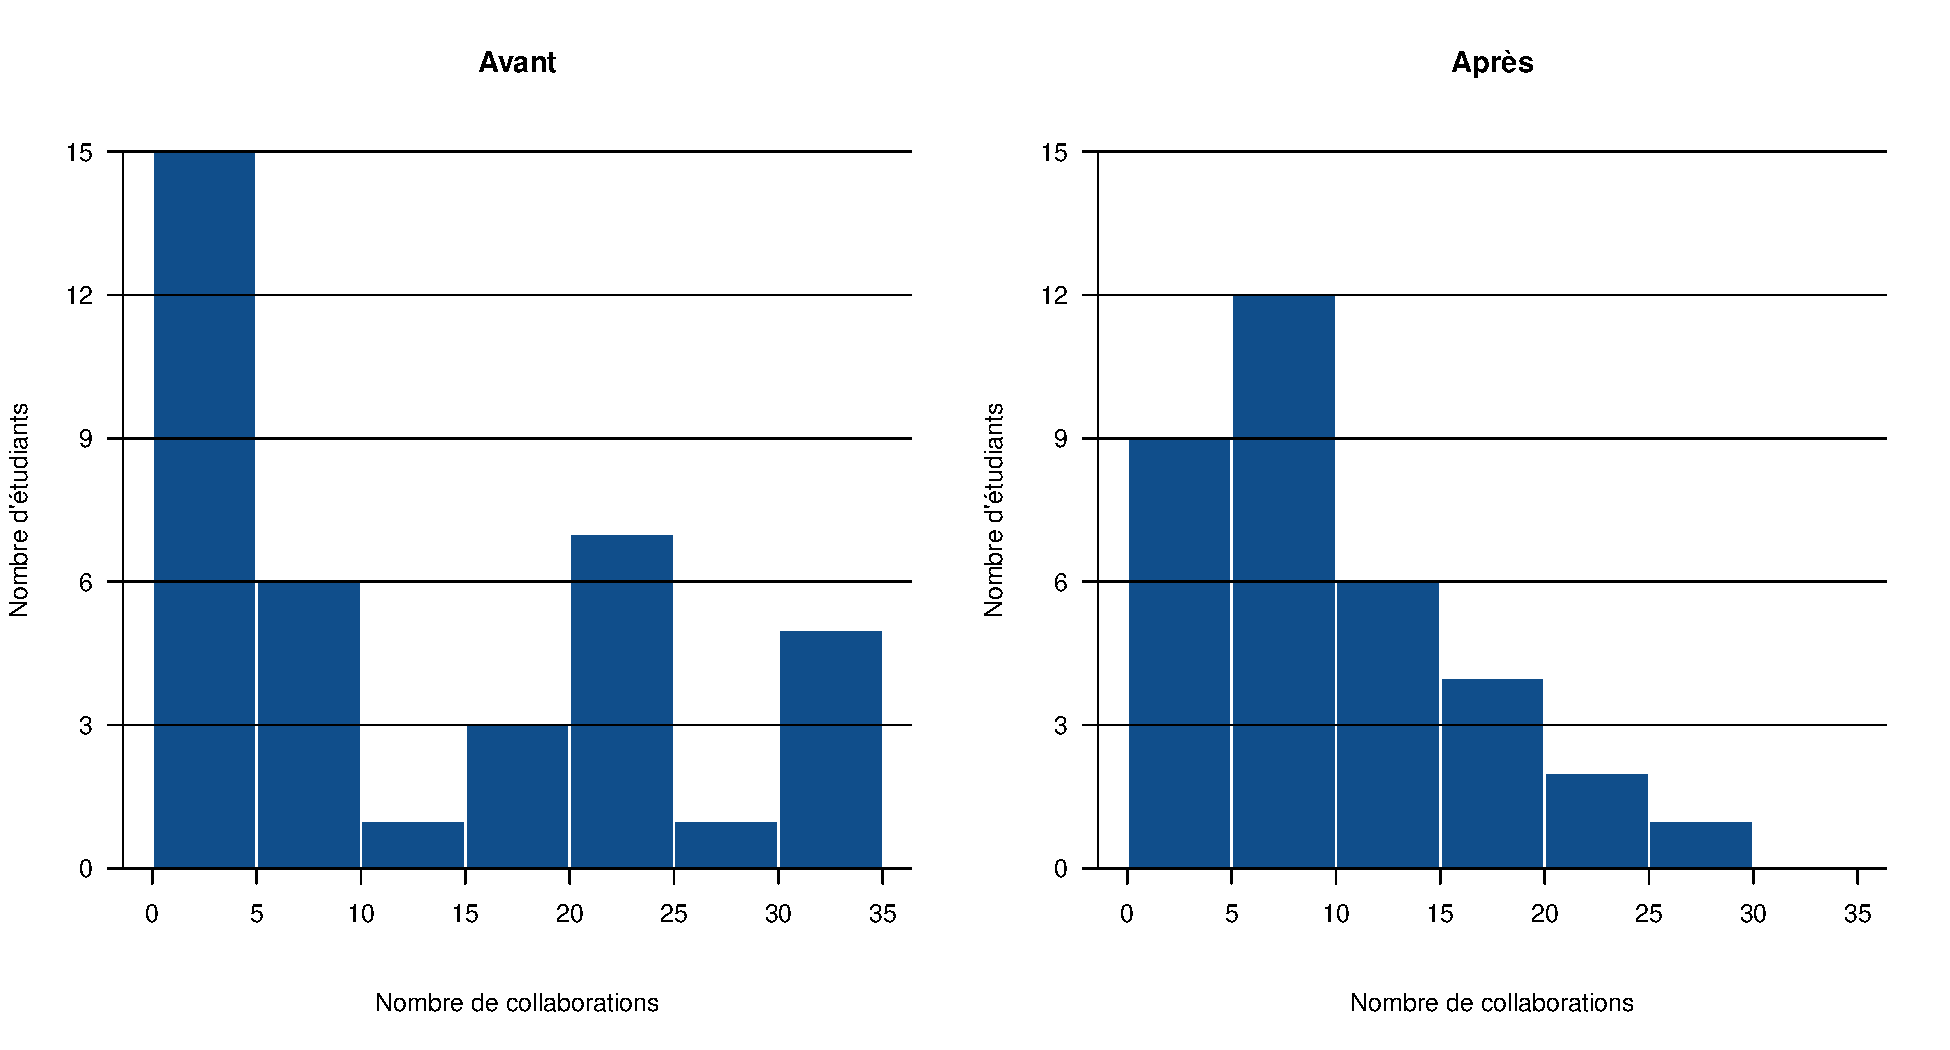
\includegraphics[width=\textwidth]{figure_avant_apres_covid.pdf}
\caption{Comparaison de la distribution du nombre de collaborations par étudiants avant et après la mise en place des mesures sociosanitaires contre la covid-19 en 2020.}
\label{fig:h}
\end{figure}

\clearpage
\bibliographystyle{apalike}
\bibliography{biblio_projet_bio500}
\end{document}
